\section{System Overview}
\label{sec:overview}

Spider I and Spider II system overview. Identifying significant changes in storage architecture.

\begin{figure}[!t]
\centering
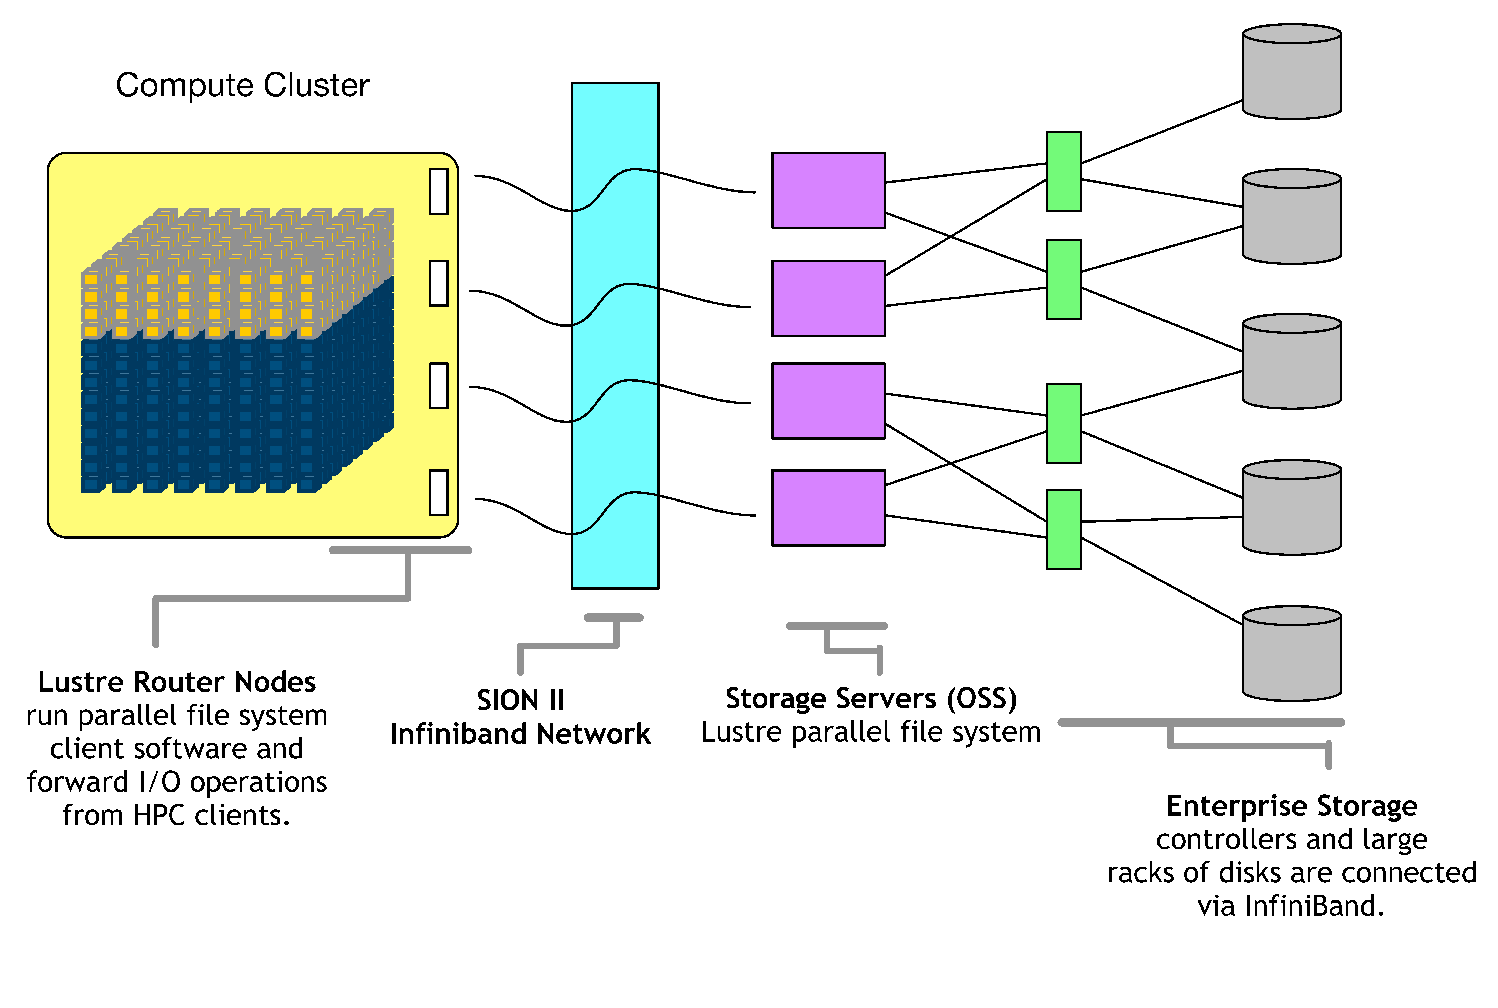
\includegraphics[width=0.45\textwidth]{./figs/spider2arch.ps}
\vspace{-0.1in}
\centering
\caption{Spider Architecture}
\label{fig:arch}
\end{figure}

\begin{table}{h!}
\begin{center}
\begin{tabular}{l||l|l}
 Spec & Spider 1 & Spider 2\\
\hline
Bandwidth & 240 GB/s & 1 TB/s \\
\
Capacity & 10 PB & 32 PB \\
Addmore \\
\end{tabular}
\end{center}
\end{table}


\subsection{Monitoring tool}
DDNTool \cite{ddntool10:ross} was developed to monitor the DDN S2A and SFA storage system RAID controllers. Since the two DDN architectures have very different monitoring API's, there are actually two completely separate programs:  DDNTool for the S2A architecture and DDNTool\_v2 for the SFA architecture.  The two tools are very different in their implementations - DDNTool is a C++ program that communicates with the disk controllers directly over TCP/IP while DDNTool\_v2 is a Python program that interfaces with a vendor-supplied python library which handles the low level communication - but they both accomplish the same basic task.  The tools poll each controller for various pieces of information (e.g. I/O request sizes, write and read bandwidths) at regular rates and store this information in a MySQL database.  The database is not actually used for long term storage.  In fact, at each poll interval, the old data is overwritten with new data.  By storing a the data in a database, though, the data is available to numerous clients via a well-documented API.  This allows multiple users to search and query in real-time.

